\chapter{Systemauswahl}
\label{chapter:systemauswahl}
Mit den unter \ref{qualitätsmetriken} erstellten Metriken sind die Frameworks GeoMesa, Postgres-XL und Rasdaman zu vergleichen.
Der Vergleich findet im Rahmen einer Nutzwertanalyse statt.
Hierbei werden keine Daten von durchgeführten Tests herangezogen, sondern es wird anhand der Spezifikation der einzelnen Frameworks untersucht ergo eine Inspektion als Prüfmethode verwendet.

\section{Definition der Nutzwertanalyse}
\label{section:definitionnutzwertanalyse}
Die drei Frameworks wurden aus der Tabelle der Abbildung \ref{fig:spatialdatabases} ausgewählt.
\begin{figure}
\centering
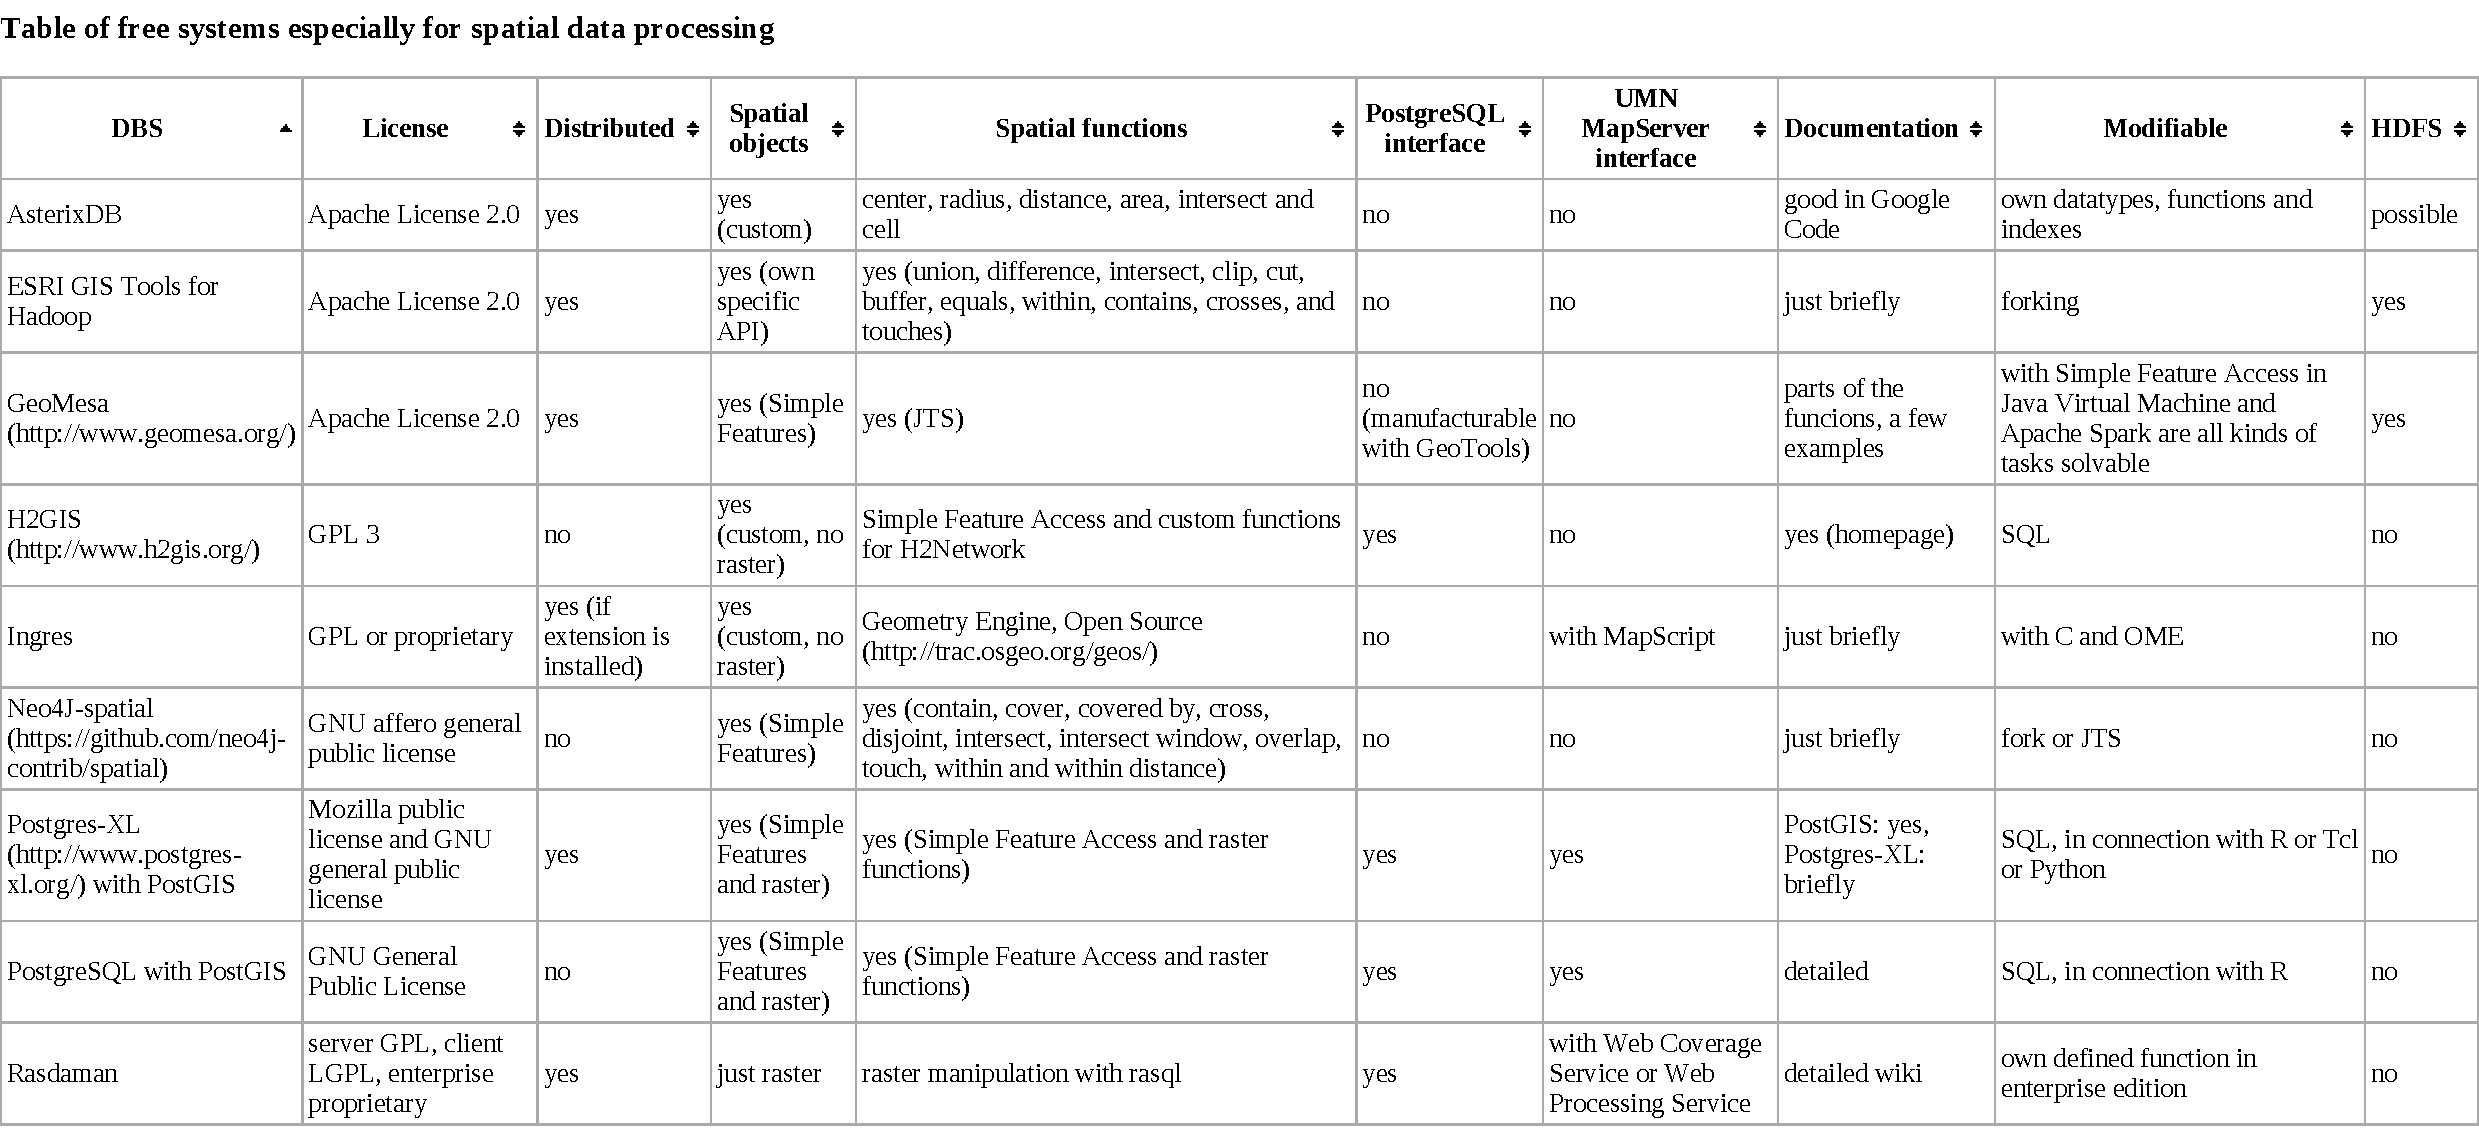
\includegraphics[angle=90,width=.66\textwidth]{Abbildungen/table_spatialdatabases_13_2_15.pdf}
\caption[Übersicht relevanter GIS Frameworks]{Übersicht relevanter GIS Frameworks nach \cite{website:wiki-spatialdatabase} vom 13.2.2015}
\label{fig:spatialdatabases}
\end{figure}
Darin sind GIS zur räumlichen Datenverarbeitung mit wesentlichen Eigenschaften wie \mbox{PostgreSQL} Schnittstelle und räumliche Datentypen aufgelistet.
Entsprechend den Anforderungen wurden daraus drei Frameworks für die Nutzwertanalyse ausgewählt.
Anforderung war dabei, dass Schnittstellen zu PostgreSQL und \Gls{umn} gegeben sind und es sich um ein Open-Source Frameworks handelt.\\
Abbildung \ref{fig:spatialdatabases} stammt von der Wikipedia Seite \url{https://en.wikipedia.org/wiki/Spatial_database} und ist für Unternehmen relevant, wie unter Kapitel \ref{aufrufe-spatialdatabases} beschrieben.
Der Autor erschuf die abgebildete Tabelle durch Recherche und stellte sie am 1.2.2015 in den Artikel.
In der Annahme, dass unternehmensbezogene Besucher der Seite fehlendes ergänzen oder falsches korrigieren würden, dient diese zur Auswahl geeigneter Frameworks.

Tabelle \ref{table:Wertungsmassstab} zeigt die für die Nutzwertanalyse notwendige Wertung der einzelnen Metriken.
Die Metriken Richtigkeit, Fehlertoleranz und Zeitverhalten werden nicht in die Analyse aufgenommen, da sie über die Spezifikation nicht belegbar sind.
\begin{table}[h!]
\centering
\begin{tabular}{l|l}
\textbf{Metrik} & \textbf{Gewichtung in \%} \\ \hline
%Richtigkeit & 10 \\ \hline
Interoperabilität & 30 \\ \hline
Funktionsumfang & 20 \\ \hline
%Fehlertoleranz & 8 \\ \hline
Dokumentation & 35 \\ \hline
%Zeitverhalten & 16 \\ \hline
Modifizierbarkeit & 15
\end{tabular}
\caption{Wertungsmaßstab der einzelnen Metriken}
\label{table:Wertungsmassstab}
\end{table}

Für jedes Framework wird eine Nutzwertanalyse durchgeführt und die dazugehörige Tabellen dazu präsentiert.
Zu jeder Metrik wird der erreichte Wert, die ungewichtete Erfüllung, die gewichtete Erfüllung und ein Kommentar angegeben.
Die ungewichtete Erfüllung bezieht sich auf den maximal zu erreichenden Wert der Metrik, die gewichtete Erfüllung dagegen auf die Erfüllung der Metrik in Bezug auf Tabelle \ref{table:Wertungsmassstab}.
Die Kommentarspalte dient der Darstellung des Erreichens der Mindestanforderungen.
Der schlussendliche Nutzwert ergibt sich nach Zangemeister in \cite{website:nutzwertanalyse} aus der Summe der Produkte des Teilnutzens des jeweiligen Kriteriums mit der Gewichtung des Kriteriums.
Der Teilnutzen ist hier der Prozentuale Anteil der erreichten Punktzahl an der maximalen Punktzahl des Kriteriums.
Diese Prozentangabe wird als Wert mit der Gewichtung des Kriteriums multipliziert, woraus sich der Nutzwert für das Kriterium ergibt.
Die Summe aller dieser Teilnutzwerte ergibt den Nutzwert des Frameworks für den Anwendungsfall.

Die granulare Bewertung der einzelnen Kriterien der drei Systeme ist im Anhang \ref{appendix:systembewertung} zu finden.

\section{Nutzwertanalyse}

\subsection{GeoMesa}
\begin{table}[h!]
\centering
\small
\begin{tabular}{l|p{1.8cm}|c|p{3.1cm}|p{1.8cm}}
\textbf{Metrik} & \textbf{erreichter Wert} & \textbf{Erfüllung in \%} & \textbf{Kommentar} & \textbf{gewichteter Teilnutzen} \\ \hline
Interoperabilität & 7 & 58 & Implementationen für beide Schnittstellen notwendig. & 17 \\ \hline
Funktionsumfang & 48 & 79 & Die meisten Funktionen sind nur mit Scala verfügbar, Mindestabdeckung jedoch gegeben. & 16 \\ \hline
Dokumentation & 4 & 31 & Mindestabdeckung nicht erfüllt. & 11 \\ \hline
Modifizierbarkeit & 4 & 80 & Mit Simple Features und Spark umfangreiche Problemlösungen erstellbar. Fehlende Funktionen können nachgerüstet werden. & 12 \\
\end{tabular}
\caption{Nutzwertanalyse GeoMesa}
\label{table:nutzwertanalyse-geomesa}
\end{table}
Der Nutzwert von GeoMesa ist nach Tabelle \ref{table:nutzwertanalyse-geomesa} 56.
Die detaillierte Analyse und Bewertung ist im Anhang \ref{appendix:systembewertung-geomesa} zu finden.
Darin waren die wichtigsten Quellen die offiziellen Webseiten von GeoMesa \cite{website:geomesa-tutorials} und \cite{website:geomesa-simplefeatures} sowie der Artikel \cite{website:geomesaeclipse}.

Neben dem messbaren Nutzwert sind die nichttechnischen Kriterien zu nennen, welche auf die Auswahl eines Frameworks Einfluss haben.
Dazu zählt die Herstellerfirma mit Marktposition, Produktplanung und Service sowie das Produkt in Hinsicht auf Preis, Lebendigkeit in Form von Entwickleraktivität und Größe der Benutzer.\\
\url{https://github.com/locationtech/geomesa} zählt am 17.2.2015 271 commits, 20 contributors und 186 branches.
Eine solche hohe Anzahl an branches spricht normalerweise für eine hohe Nutzung und Lebendigkeit des Projektes.
Jedoch wurde die Mehrzahl der branches nicht in den master Zweig übernommen.
\begin{figure}[h!]
\centering
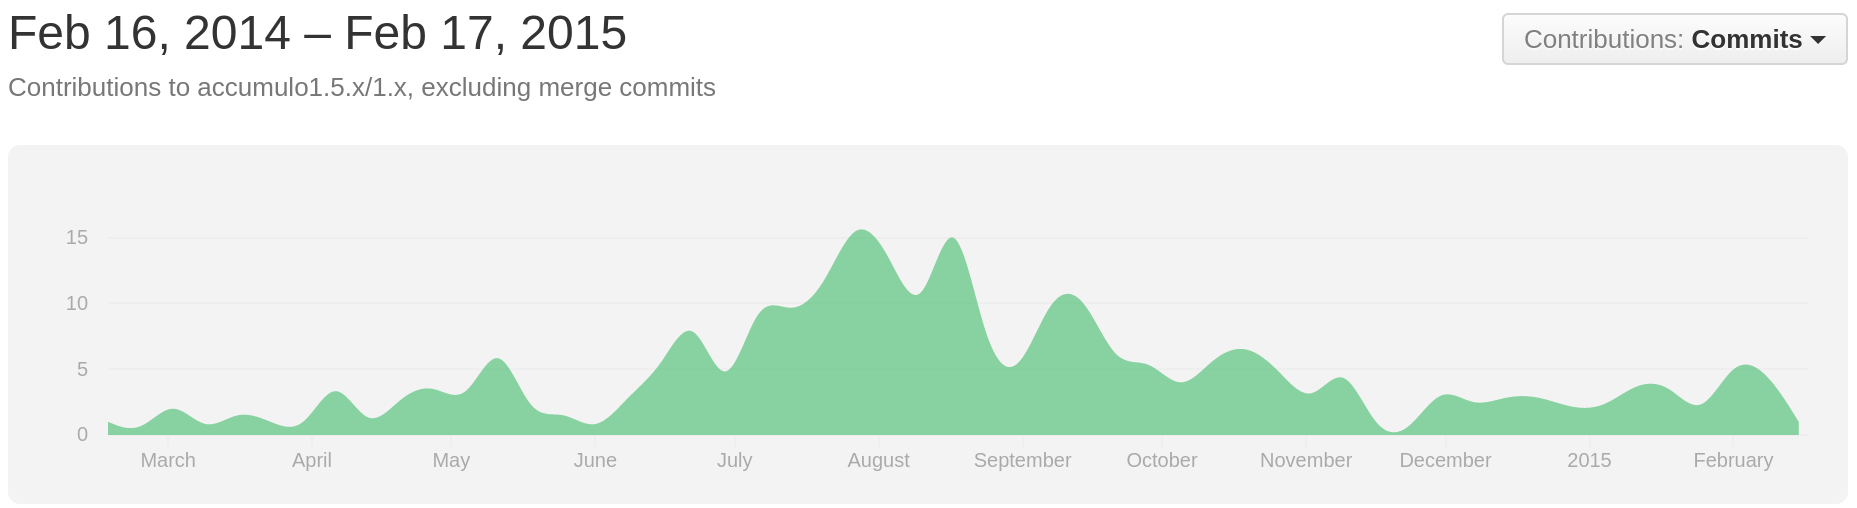
\includegraphics[width=\textwidth]{Abbildungen/geomesa_timeline_contributors.png}
\caption[Zeitleiste der contributor von GeoMesa]{Zeitleiste der contributor von GeoMesa vom 17.2.2015 nach \url{https://github.com/locationtech/geomesa/graphs/contributors}}
\label{fig:timeline_contr_geomesa}
\end{figure}
\begin{figure}[h!]
\centering
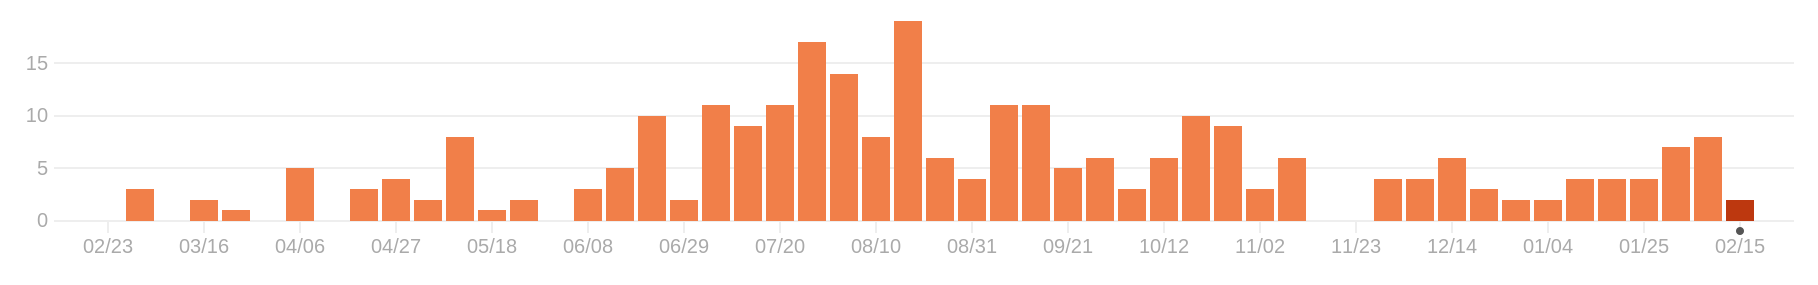
\includegraphics[width=\textwidth]{Abbildungen/geomesa_timeline_commits.png}
\caption[Zeitleiste der commits von GeoMesa]{Zeitleiste der commits von GeoMesa vom 17.2.2015 nach \url{https://github.com/locationtech/geomesa/graphs/commit-activity}}
\label{fig:timeline_commits_geomesa}
\end{figure}
Das GeoMesa Projekt auf GitHub hat nach Abbildung \ref{fig:timeline_contr_geomesa} eins bis vier Stammprogrammierer und ist im zweiten und dritten Quartal gegenüber mit der doppelten Anzahl an contributors gegenüber den anderen Quartalen fragmentiert.
Die drei contributors mit dem größten Anteil an Änderungen sind vorwiegend in Projekten von LocationTech aktiv was darauf schließen lässt, dass sie für das Unternehmen arbeiten.
Daraus folgt das zum wesentlichen Teil das Unternehmen LocationTech das Projekt wartet.
Die Anzahl der commits geht mit dem Verlauf der aktiven Programmierer einher.
Abbildung \ref{fig:timeline_commits_geomesa} zeigt die selbe Quartalsweise Verteilung wie Abbildung \ref{fig:timeline_contr_geomesa}.
Dabei ist der Unterschied zwei zu neun commits pro Woche.

LocationTech ist eine Arbeitsgruppe der non-for-profit Stiftung Eclipse.
In diesem Rahmen erhält diese Arbeitsgruppe 20 Mitglieder für Projektplanung und Projektumsetzung.
Weiterhin findet die Finanzierung im Rahmen von Mitgliedschaft an der Arbeitsgruppe statt.
Darin können Mitglieder je nach Beitrag Teile der Entscheidungsorgane der Arbeitsgruppe werden und Zugang zu Ergebnissen dieser erhalten. \cite{website:locationtech-about}
LocationTech ist mit GeoMesa mitten in der Entwicklung und hat keine permanenten aktive Unterstützer.
Dieser Stand spricht gegen eine Auswahl von GeoMesa zum produktiven Einsatz.

\subsection{Postgres-XL}
\label{gegenuerbestellung:postgresxl}
\begin{table}[h!]
\centering
\small
\begin{tabular}{l|p{1.8cm}|c|p{3.1cm}|p{1.8cm}}
\textbf{Metrik} & \textbf{erreichter Wert} & \textbf{Erfüllung in \%} & \textbf{Kommentar} & \textbf{gewichteter Teilnutzen} \\ \hline
Interoperabilität & 12 & 100 & Analog des Ist-Standes. & 30 \\ \hline
Funktionsumfang & 53 & 87 & Mindestabdeckung erfüllt, jedoch sind Geostatistik und Versionierung nicht vorhanden. & 17 \\ \hline
Dokumentation & 9 & 69 & Dokumentation zu PostGIS ist sehr gut, zu Postgres-XL grob. Mindestabdeckung ist erfüllt. & 24 \\ \hline
Modifizierbarkeit & 5 & 100 & Vollständige Abdeckung vorhanden. Möglichkeiten sind in SQL gegeben. & 15 \\
\end{tabular}
\caption{Nutzwertanalyse Postgres-XL}
\label{table:nutzwertanalyse-postgresxl}
\end{table}
Aus Tabelle \ref{table:nutzwertanalyse-postgresxl} ergibt sich ein Nutzwert von 86.
Das Ergebnis bezieht sich auf Anhang \ref{gegenuerbestellung:postgresxl}.
Es wurde vorrangig die Postgres-XL Dokumentation \cite{website:postgresxl-manual} und jene von PostGIS \cite{website:postgisdocu-functions} verwendet.

Dazu sind ebenso nichttechnische Faktoren zu berücksichtigen.\\
\url{https://github.com/snaga/postgres-xl} zählt am 17.2.2015 35.266 commits, 23 contributors und drei branches.
\begin{figure}[h!]
\centering
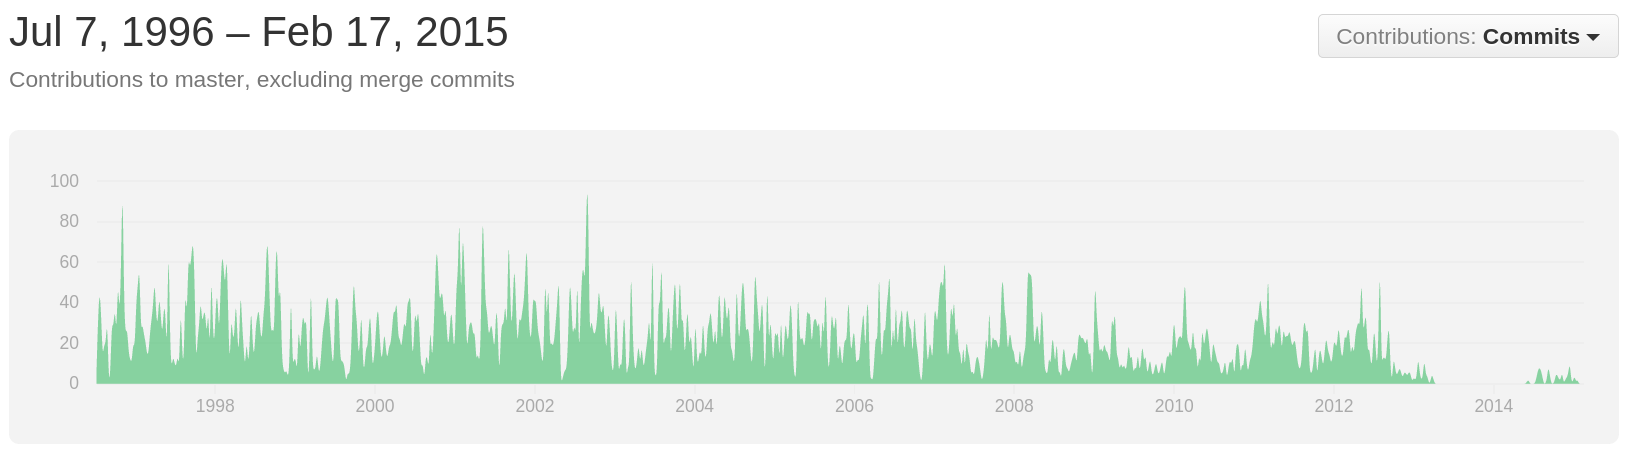
\includegraphics[width=\textwidth]{Abbildungen/postgresxl_timeline_contributors.png}
\caption[Zeitleiste der contributor von Postgres-XL]{Zeitleiste der contributor von Postgres-XL vom 17.2.2015 nach \url{https://github.com/snaga/postgres-xl/graphs/contributors}}
\label{fig:timeline_contr_postgresxl}
\end{figure}
\begin{figure}[h!]
\centering
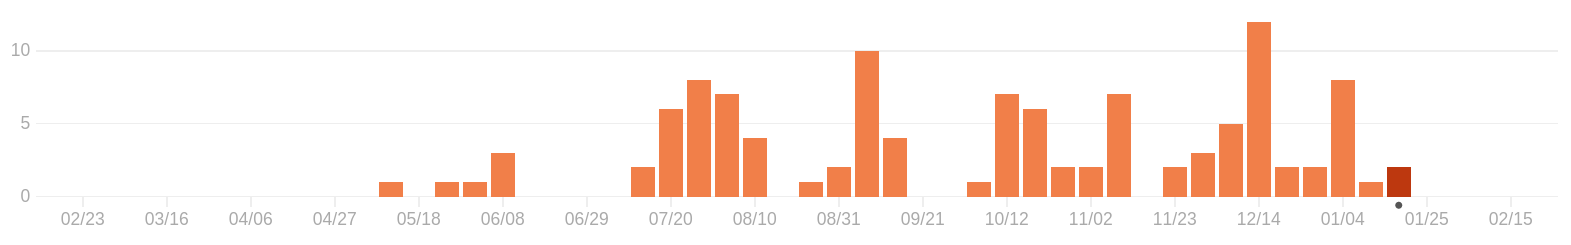
\includegraphics[width=\textwidth]{Abbildungen/postgresxl_timeline_commits.png}
\caption[Zeitleiste der commits von Postgres-XL]{Zeitleiste der commits von Postgres-XL vom 17.2.2015 nach \url{https://github.com/snaga/postgres-xl/graphs/commit-activity}}
\label{fig:timeline_commits_postgresxl}
\end{figure}
Abbildung \ref{fig:timeline_contr_postgresxl} zeigt einerseits, dass dieses Projekt seit 1998 besteht, andererseits das die Zahl der aktiven contributors im Gegensatz der Jahre 1998 bis 2012 zu 2014/2015 in etwa ein viertel beträgt.
Diese deutliche abrupte Abnahme der aktiven Programmierer deutet eine Veränderung im Projekt oder den Projektverantwortlichen an.
Die commits des vergangenen Jahres sind in Abbildung \ref{fig:timeline_commits_postgresxl} dargestellt.
Danach wurden im ersten Halbjahr 2014 nur insgesamt 6 commits und im zweiten Halbjahr 2014 etwa täglich ein commit durchgeführt.

Das Unternehmen TransLattice\footnote{\url{http://www.translattice.com/}} übernahm im Mai 2014 das Unternehmen StormDB.
Die Übernahme schloss das Projekt Postgres bzw. Postgres-XC ein. (siehe \cite{website:translattice-stormdb})
Dieses wurde darauf in Postgres-XL umbenannt und erweitert.
Diese Änderung rief die Verringerung der contributors seit Anfang 2014 hervor.
TransLattice verwaltet seitdem das Projekt und stellt technischen sowie theoretischen Support.
Postgres-XL ist durch die langjährige Entwicklung empfehlenswert für den produktiven Einsatz.
Jedoch ist die Aktivität der TransLattice Entwickler zu beobachten, da die Gefahr besteht das dieses Projekt vom Unternehmen nicht mehr gefördert wird und somit Fehler und Verbesserungen nicht eingepflegt werden und neue PostgreSQL Versionen nicht unterstützt werden.


\subsection{Rasdaman}
\begin{table}[h!]
\centering
\small
\begin{tabular}{l|p{1.8cm}|c|p{3.1cm}|p{1.8cm}}
\textbf{Metrik} & \textbf{erreichter Wert} & \textbf{Erfüllung in \%} & \textbf{Kommentar} & \textbf{gewichteter Teilnutzen} \\ \hline
Interoperabilität & 7 & 58 & \Gls{umn} Schnittstelle ist nicht vorhanden. & 17 \\ \hline
Funktionsumfang & 10 & 16 & Umfangreiche Rasterverarbeitung möglich. Kostenlose Version enthält keine Optimierungen. Abbildung von Simple Features auf Arrays mit Aufwand verbunden und nur bedingt sinnvoll. Mindestabdeckung wird nicht erfüllt. & 3 \\ \hline
Dokumentation & 8 & 62 & Mindestabdeckung erfüllt. & 22 \\ \hline
Modifizierbarkeit & 3 & 60 & Einfache Java und C++ API bietet zwar Erweiterungsmöglichkeiten, aber die Mindestabdeckung ist durch fehlende Datentypen nicht gegeben. & 9 \\
\end{tabular}
\caption{Nutzwertanalyse Rasdaman}
\label{table:nutzwertanalyse-rasdaman}
\end{table}
Aus Tabelle \ref{table:nutzwertanalyse-rasdaman} ergibt sich ein Nutzwert von 51.
Die granulare Bewertung befindet sich im Anhang \ref{appendix:systembewertung-rasdaman}.
Als Quelle diente dabei \cite{website:rasdaman-features} mit verlinkten Websites des gleichem Domain Namen.

Die Statistiken der Entwicklung des Repository müssen händisch gewonnen werden, da es auf einem Trac Verwaltungssystem mit Git basiert.
Das Repository ist unter\\\url{kahlua.eecs.jacobs-university.de/rasdaman.git} verfügbar.
Es kann mit der Konsolenanwendung Git heruntergeladen und ausgewertet werden.
So erhält man mit \textit{git log --pretty=format:\grqq \%h - \%an, \%ad : \%s\grqq\ | tail -1} das der erste commit 2009 erstellt wurde:
\begin{quote}
0f1055b - Constantin Jucovschi, Tue Mar 31 06:18:54 2009 -0400 : Initial commit
\end{quote}
Somit sind auch die commits des vergangenen Jahres ermittelbar.
So wurden vom 19.2.2014 bis zum 19.2.2015 1949 commits durchgeführt.
\textit{git shortlog -sne} liefert dagegen alle Autoren der vorhandenen commits.
Die Autoren der meisten commits sind Dimitar Misev mit 456, Piero Campalani mit 301 und Andrei Aiordachioaie mit 74 commits, Stand 19.2.2015 14:00 Uhr.
Herr Misev ist %laut seinem Linkedin Profil auf\\\url{https://de.linkedin.com/in/dimitarmisev}
Director of Product Development der \mbox{rasdaman} GmbH.
Herr Campalani und Herr Aiordachioaie haben wie Herr Misev an der Jacobs Universität in Bremen studiert, arbeiten aber nicht bei der \mbox{rasdaman} GmbH.

Rasdaman ist laut der Meldung \glqq Führender Rasterserver kostenfrei zum Download\grqq\ in \cite{website:rasdaman-newsarchive} seit September 2008 in einer freien Version verfügbar.
Außerdem ist es aus Forschungsarbeiten der TU Darmstadt, der TU München und der Jacobs University Bremen entstanden.
Förderer war dabei das Community Research and Development Information Service der EU. \cite{website:rasdaman-cordis}

\section{Zusammenfassung}
%Auf Hypothese zu sprechen kommen - durch hinreichenden Informationsgehalt und empirische Beobachtungen bewiesen
Auf Grund der Ähnlichkeit von Postres-XL zum Ist-Stand erfüllt es nicht nur alle Mindestanforderungen, sondern erzielt auch den höchsten Nutzwert der untersuchten Frameworks.
Der Nutzwert von 86 ist auf 86\% Erfüllung der untersuchten Qualitätsmetriken abbildbar.
Da die Anforderungen neben vorhandenen Qualitäten des Ist-Standes fehlende dessen enthalten, betont diese hohe Erfüllung die Eignung für zukünftige Anforderungen an Zeitverhalten und Modifizierbarkeit.
Weiterhin spricht die Existenz seit 1996 für Postgres-XL.
Einzig die Übernahme der Firma TransLattice und der damit einhergegangene Einbruch der Anzahl an commits und contributors ist negativ und für die Zukunft zu beobachten.

GeoMesa und Rasdaman sind für andere spezielle Anwendungsfälle geeignet.
So ist Rasdaman in der kommerziellen Version bei verteilter Rasterdatenverarbeitung zu empfehlen.
GeoMesa eignet sich auf Grund des BigTable Ansatzes für enorm große Datenmengen die im Peta Bereich liegen.
So können diese Daten nicht nur gespeichert, sondern auch mit Scala und dazugehörigen Frameworks und Bibliotheken verteilt und parallel nach selbst erstellten Algorithmen und Vorgängen verarbeitet werden.

Die Systemauswahl hat nicht nur ein geeignetes Framework als Ergebnis, sondern auch ein Grundgerüst zur Beurteilung anderer Frameworks und Anwendungsfälle anhand von Nutzwertanalysen.
In Folge ist Postgres-XL detailliert zu untersuchen und erneut zu bewerten.